%%
%% This is file `example-1.tex',
%% generated with the docstrip utility.
%%
%% The original source files were:
%%
%% drexel-thesis.dtx  (with options: `example-part')
%% 
%% This is a generated file.
%% 
%% Copyright (C) 2010 W. Trevor King
%% 
%% This file may be distributed and/or modified under the conditions of
%% the LaTeX Project Public License, either version 1.3 of this license
%% or (at your option) any later version.  The latest version of this
%% license is in:
%% 
%%    http://www.latex-project.org/lppl.txt
%% 
%% and version 1.3 or later is part of all distributions of LaTeX version
%% 2003/06/01 or later.
%% 

\chapter{Methods}

\section{Neuron model}
Computational neuroscience makes use of a number of neuron models.
By far the most common model used when studying traveling waves and other mesoscopic behavior is the leaky integrate-and-fire neuron.
The computational efficiency of the LIF model has allowed researchers to simulate large numbers of neurons over time scales of seconds or minutes.
However this computational efficieny comes at the cost of accurate representation of internal neuron dynamics.
\\
The LIF equations model a single neuron variable, the membrane potential, in a single differential equation (Eq \ref{eq:lif}).
The Izhikevich model includes an additional variable that represents a collection of ionic mechanisms and uses two coupled differential equations.
This two-dimensional model can capture a number of biologically observed dynamical phenomenon not possible in a one-dimensional model while still being computationally efficient.
\\
Critical phenomenon observed in the Izhikevich model and not the LIF model include variable firing rates, post-inhibitory rebound spiking and delayed spiking.
Plots: LIF vs Izzy post-inhibitory rebound spiking, delayed spiking, 

To study traveling waves in small columnar ensembles (SCE) of neurons we created a MATLAB simulation of our model based on \citet{izhikevich2003}.
We model the firing dynamics of each neuron using the Izhikevich model \citep{izhikevich2003} that consists of a two-dimensional model of two coupled differential equations given by:
\begin{align}
 \begin{split}
  v^\prime &= 0.04v^2+5v+140-u+I \label{eq:neuron_v} \\
  u^\prime &= a(bv-u)
 \end{split}
\end{align}
where $v$ is the membrane potential of the neuron and $u$ is a membrane recovery variable, with a spike threshold and an auxilliary after-spike resetting of parameters by:
\begin{align}
  \text{if } &v>30: v\leftarrow c, u\leftarrow u+d
\end{align}
and I is the sum of all incoming currents to the neuron, explained in detail below. 

Equation \ref{eq:neuron_v} has four parameters (a,b,c,d) that with specific values can model a wide range of neuronal spiking behavior \citep{izhikevich2003}. 
The parameters used here (see Table \ref{tab:izzy_params}) are based on the original model with modification of the $c$ parameter for excitatory neurons and define a random population of neurons where $U(s,t)$ represent a number drawn from a uniform random distribution between s and t. 
\begin{table}[!htb]
 \caption{Izhikevich model parameters}
 \label{tab:izzy_params}
 \centering
 \begin{tabular}{lcr}
  \textbf{Parameter} & \textbf{Excitatory} & \textbf{Inhibitory} \\
  \hline
  a & 0.02 & 0.02+$\mathcal{U}$(0,0.08) \\
  b & 0.2 & 0.25-$\mathcal{U}(0,0.05)$\\
  c & -65+$\mathcal{U}(0,10)^2$ & -65 \\
  d & 8-$\mathcal{U}(0,6)$& 2 \\
 \end{tabular}
\end{table}
For solving equation \ref{eq:neuron_v} numerically we use the modified Euler method from \citet{izhikevich2003} with a time step of $0.2 ms$ except were noted. 

The current I in equation \ref{eq:neuron_v} includes the sum of all incoming stimuli into neuron $i$ from other neurons $I_i$ and external stimuli $I_{i,e}$ applied to the system. 
The neuron-neuron incoming current $I_i$ into neuron $i$ is given by:
\begin{align}
 I_i(t) &= \sum_{j\ne i} \sum_{t^\prime_j} S_{ij}  \Theta(t-t^\prime_j-\tau_{ij})e^{-(\frac{t-t^\prime_j-\tau_{ij}}{\sigma_s})^2}
\end{align}

where $t'_j$ are the firing times of neuron $j$, $\Theta$ is the Heaviside step function, and the exponential factor models an exponentially decaying synapse response with a time constant of $\sigma_s = 4 ms$. 
The $S_{ij}$ represent the connection strengths between presynaptic neuron $j$ and postsynaptic neuron $i$ given by
\begin{align}
 \begin{split}
  S_{ij}^{excitatory} &= K \times \mathcal{U}\{0,0.5 \} \\
  S_{ij}^{inhibitory} &= K \times \mathcal{U}\{-1,0 \}  \\
 \end{split}
\end{align}
where $K$ is a parameter that modulates the strength of connections, with $K=1$ corresponding to the original model in \citet{izhikevich2003}. 

The distribution of Izhikevich model parameters results in variations between our excitatory and inhibitory neurons, as well as variation in the neurons within those classes.
We examine the inter-spike interval (ISI) and its inverse, the spike frequency, for the excitatory and inhibitory neurons in our model.
We generate 1600 excitatory or inhibitory neurons and drive them with a constant stimulus, measuring the resulting ISI/spike rate as shown in Figure \ref{fig:ISIstatistics}.
The inhibitory neurons spike at a lower input level and the spike rate rises more quickly with stronger input.
Due to the stochastic variation in the 'b' parameter for inhibitory neurons, different inhibitory neurons can have a different minimum firing threshold.
Starting at an input magnitude of $4\ mV$, at which all the inhibitory neurons fire, the spike rate of the inhibitory neurons increase linearly with the input magnitude with a slope of 13.
The excitatory neurons all have a common firing threshold.
The spike rate of the excitatory neurons increases linearly with the input magnitude, and the slope of the linear fit is 3.
\begin{figure}[!htb]
  \subfloat[][]{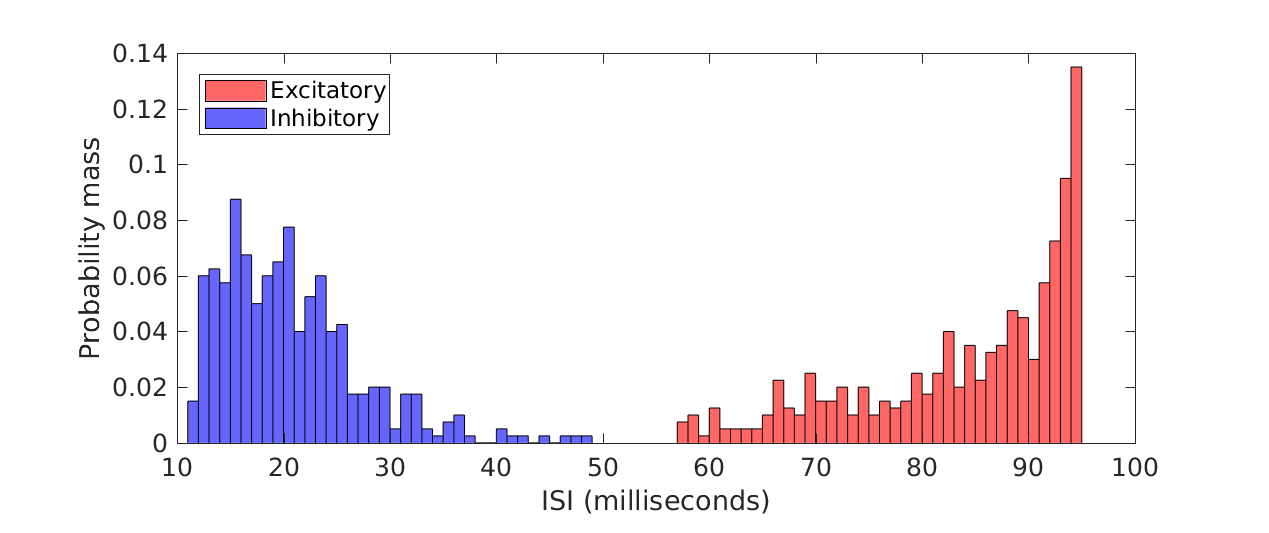
\includegraphics[width=0.75\textwidth]{fig/ISIDistribution} } 
  \subfloat[][]{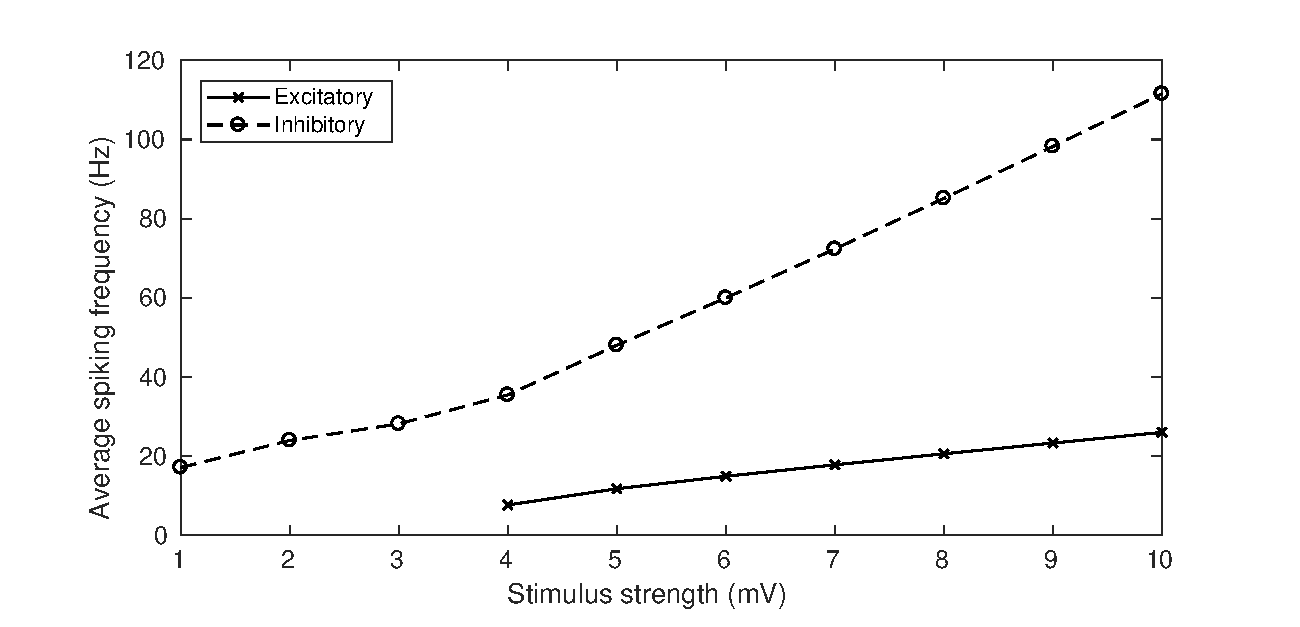
\includegraphics[width=0.75\textwidth]{fig/AvgSpikeFrequency} }
  \caption{a) The distribution of inter-spike intervals for our excitatory and inhibitory neurons with a constant $5\ mV$ stimulus.  
      b) The spike frequency of the excitatory and inhibitory neurons increases as the constant stimulus becomes stronger.}
  \label{fig:ISIstatistics}
\end{figure}
\FloatBarrier

\section{Neuron stimulus}
To drive the firing dynamics and create traveling waves we provide stimulation to the systems by using two different and separate external stimulus currents, $I_{i,e}$. 
One of them is a uniform background stimulus applied to each neuron $k$ that depends on whether the neuron is excitatory or inhibitory.
The stimulus values are drawn from a random distribution every $1 ms$ according to:
\begin{align}\label{eq:randomstim}
 \begin{split}
  I_k^{excitatory} &= M \times \mathcal{U}\{0,1 \} \\
  I_k^{inhibitory} &= \frac{2}{5} M \times \mathcal{U}\{0,1 \}
 \end{split}
\end{align}
where $M$ is a parameter that tunes the overall strength of the stimulus, with $M=5$ corresponding to the original model in \citep{izhikevich2003}. 
This stimulus has the effect of creating waves that originate from any point along an SCE and one of the uses is to study interactions between multiple waves in section \ref{sub:wave_initiation}.

The other external stimulus $I_{i,e}$ is a short constant input of current applied to all of the neurons in one area of a system.
This stimulus is used to measure wave speed and is described in section \ref{sec:wave_speed_method}.

\section{Neuron connectivity}
We first construct these assemblies by placing neurons at the vertices of a cubic lattice with coordinates X, Y and Z. 
Each neuron is  randomly chosen to be  either excitatory (E) or inhibitory (I), with the fraction of excitatory neurons indicated as $P_{exc}$.
After placing, we connect two neurons based on their relative distance according to a connection probability that favors local connectivity given by \citep{maass2002}: 
\begin{align}\label{eq:connectivity}
 P_{a,b} &= C e^{-(D(a,b)/\lambda)^2}
\end{align}
where $D(a,b)$ is the Euclidean distance between neuron a and b, $\lambda$ is the characteristic length of the local connectivity neighborhood, and $C$ is the peak probability of connection .
This local ceopnnectivity model has been observed in the mouse visual cortex\citep{Hellwig2000} and auditory cortex\citep{Levy2012}.
Multiple connections from the same presynaptic neuron to the same postsynaptic neuron, as well as self-connections, are prohibited.
Two neurons may be recurrently connected, however. 

\section{Model summary}
We summarize our model parameters in Table \ref{tab:all_params}. 
\begin{table}[!htb]
 \caption{Model Summary}
 \label{tab:all_params}
 \centering
 \begin{tabular}{c}
  \textbf{Model} \\
  \hline \\
 \end{tabular} \\
 \begin{tabular}{ll}
  Population & Excitatory, inhibitory \\
  Topology & Quasi 1-D minicolumn, quasi 2-D sheet, ``2.5D'' forest of minicolumns \\
  Connectivity & Stochastic, $P_{connect}$ exponentially decays with distance between neurons \\
  Neuron model & Izhikevich model with distribution of neuron parameters \\
  Synapse response & Exponential synaptic response with randomized peak connection strength  \\
  Spike propagation & Delay proportional to distance, Fixed propagation time \\
  Input & Random input to all neurons, Fixed stimulus to neurons at the bottom of the SCE \\
 \end{tabular}
\end{table}

\section{Wave analysis}
For every simulation we record all of the spikes from all neurons. 
We visualize the spikes in spike raster plots (e.g. Figure \ref{fig:sigma_raster} ).
For quasi one-dimensional minicolumns we focus on traveling waves in the Z direction so we plot the spikes according to the Z position of the neurons.
As a consequence, at each Z position there are multiple neurons that could contribute to the spike raster plot at that Z coordinate (e.g. 4 neurons for the X=2, Y=2 minicolumn case).
For quasi two-dimensional sheets and forests we focus on traveling waves in the X/Y plan so we plot the spikes according to the X/Y positions of the neurons.
Therefore multiple neurons can again contribute to the spike raster at a given X/Y location on the plot.

For our quasi one-dimensional minicolumns we use an automated wave detection, identification and analysis method.
To automatically identify waves in the minicolumn we perform a spatial clustering operation to the spike data to identify spatiotemporal regions identified by high firing density. 
The clustering operation produces an output cluster for any group of more than $3$ spike events that fall within a $20ms$ time window from neurons that are no more than $3$ layers apart.
Each cluster $C(t,z)$ has a time $t$ and position $z$.
This clustering removes random background firing activity. 
The waves are identified using a plane sweep algorithm that proceeds along the dimension of simulation time and applies wave labels to clusters such that all clusters with the same label are part of the same wave.
When a new cluster $C(t,z)$ is encountered, the algorithm associates $C(t,z)$ with any existing wave if the existing wave contains a cluster $C(t_c,z_c)$ within $40~ms$ and $6$ units of the new cluster.
If there is no such adjacent cluster a new wave is created using $C(t,z)$ as the first cluster.
An example of the clustering and identification is shown in Figure 2, with further illustration in SI Figure 1.

\begin{figure}[!htb]
  \centering
  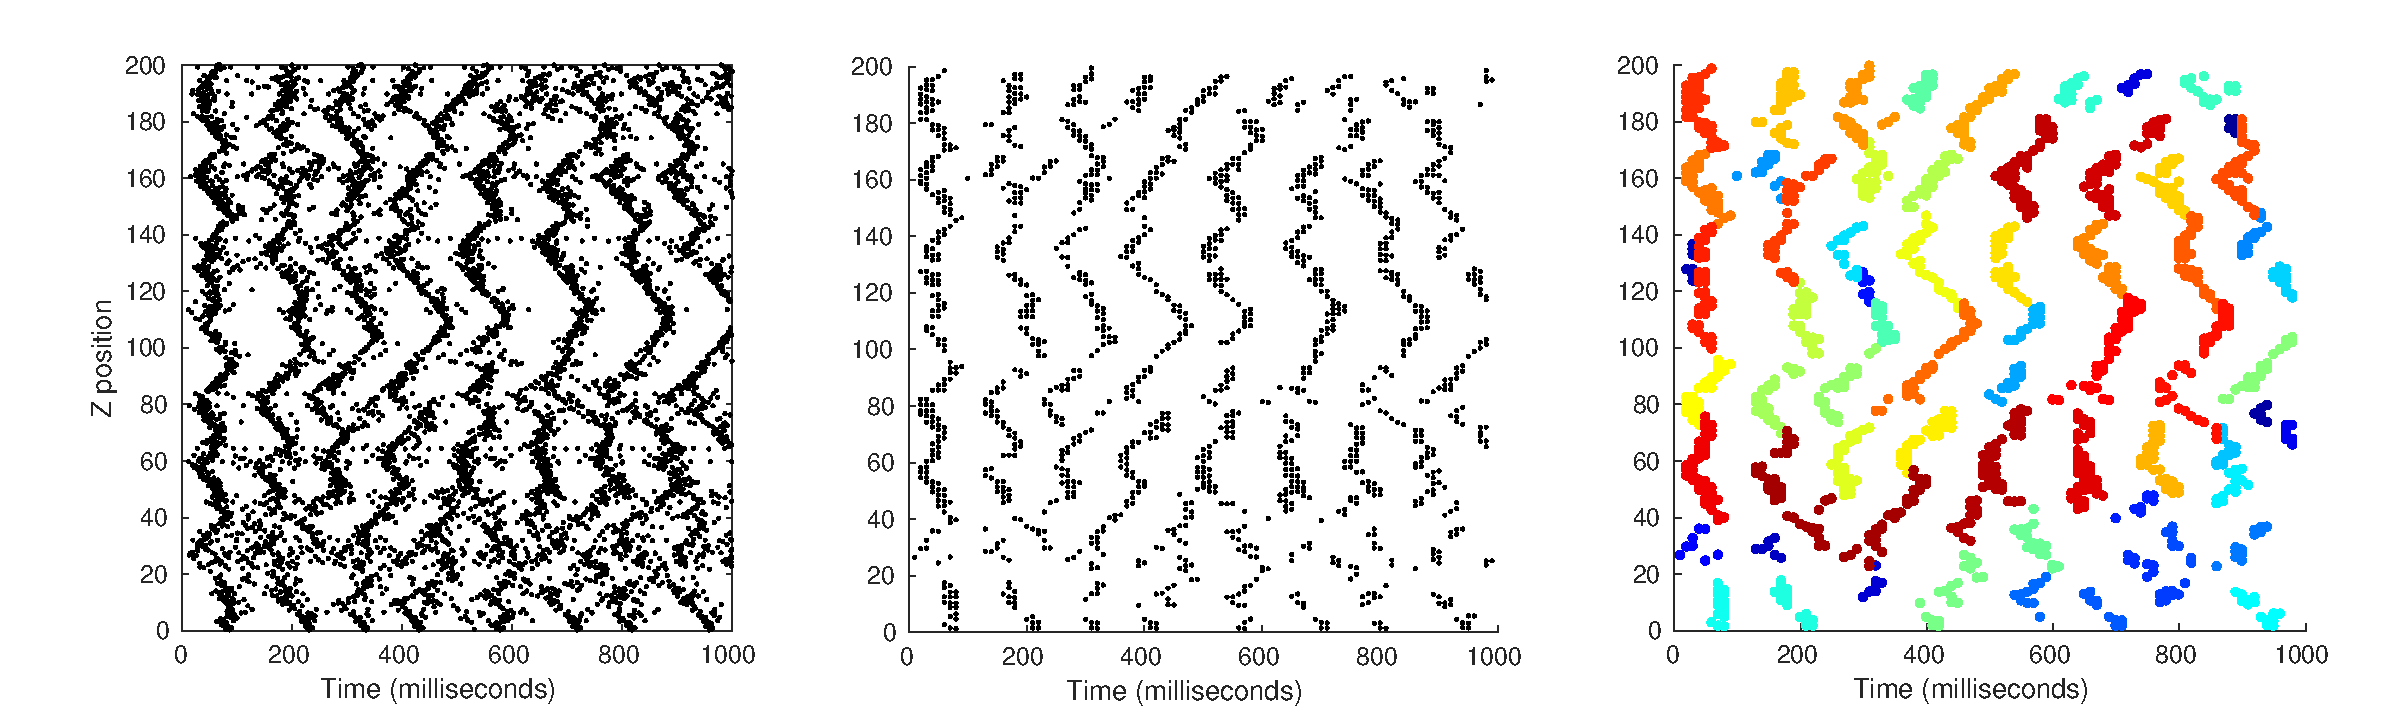
\includegraphics[width=\textwidth]{fig/DetectorExample}
  \caption{Wave identification and labeling using an example SCE with dimensions 2x2x200 . Left: Raster plot of firing events where dots represent neuronal action potentials. 
	Traveling waves can be seen as diagonal structures of dense firing activity. 
	Center: The clustering operation removes background spikes. 
	Right: Individual waves are labeled with unique identifiers color coded in the figure.}
  \label{fig:wave_analysis}
\end{figure}
\FloatBarrier

Our wave detection and analysis approach must remain valid across a range of model parameters. 
We show sample visualizations for varying values of $K$ in Figure \ref{fig:detector_test}.
This detector test demonstrates that our detection and analysis method detects and labels traveling waves of various lengths even in a noisy background.
\begin{figure}[!htb]
 \centering
   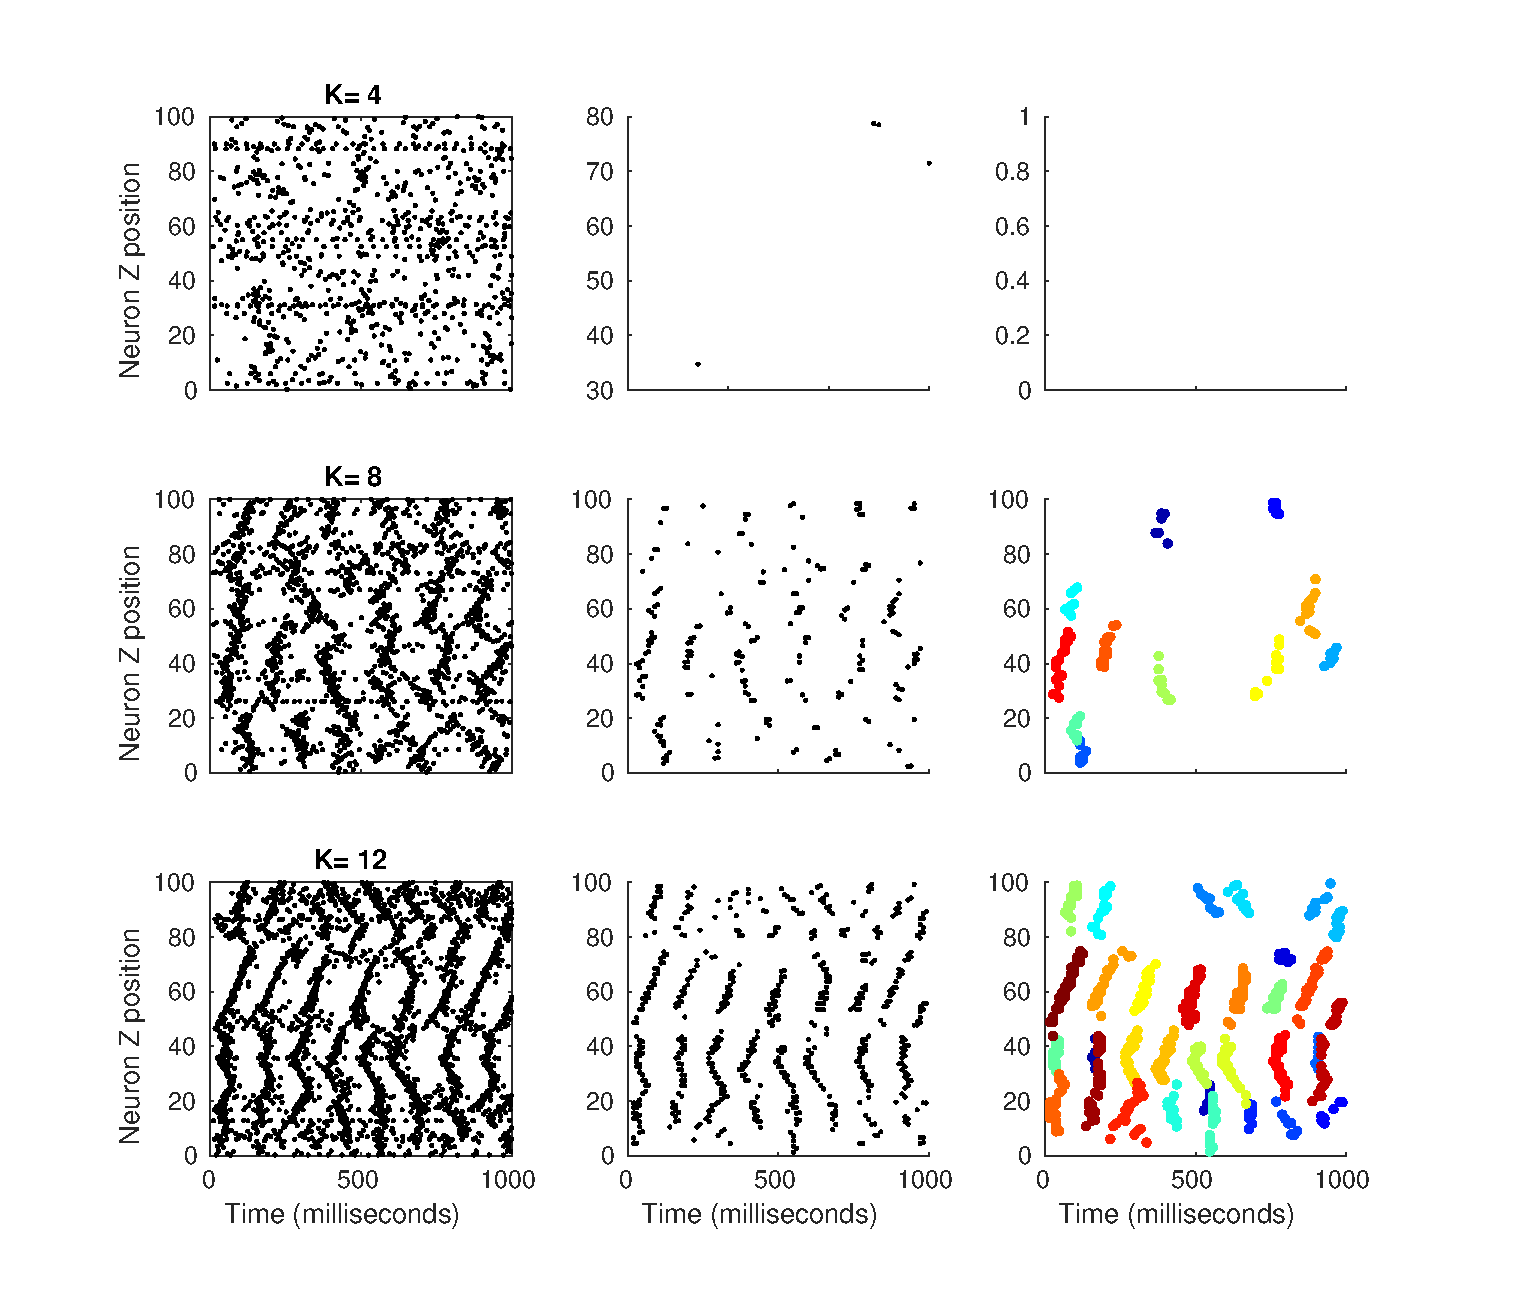
\includegraphics[width=\textwidth]{fig/DetectorTest}
    \caption{The clustering and wave labeling process. Spike raster plot (left), filtered clusters (middle) and labeled waves (right, each color is a unique wave) 
	    are shown for SCE with different values of $K$. }
  \label{fig:detector_test}
\end{figure}

\FloatBarrier
Once identified and labeled, we measure wave propagation speeds and wave initiation locations. 
We also measure the "wave firing fraction" defined as the fraction of spikes that are associated with the labeled traveling wave (total number of spikes found within the waves divided by number of spikes in the simulation). 

For the quasi two-dimensional sheets and forests we also visualize traveling waves with color plots of the membrane potential (see for example \ref{fig:2D_waves}).
The membrane potential at at X/Y position is averaged across all neurons at that position over a $2~ms$ window.
A $5x5$ smoothing filter is applied to the resulting image to improve the visibility of the wave fronts. 
For two dimensional waves we show a sequential series of these plots to illustrate the two dimensional wave behavior.

\section{Wave speed measurements}\label{sec:wave_speed_method}
To measure wave speeds we apply a constant stimulus $I_{i,e}$ over a short time period to a local area of the system.
There is no stimulus to the other neurons in the system.
This short stimulus initiates a single traveling wave that spans the entire system.
The wave arrival time is measured at some reference point in the system, and the wave speed is calculated from the wave arrival time and the distance the wave travels.

For the minicolumn system $I_{i,e}$ has a magnitude of $5$ units and is applied to the lowest $10$ layers of the minicolumn for $20~ms$.
The one-dimensional waves travel in the Z direction and the wave arrival time is measured at the top of the minicolumns.
For the two-dimensional sheet $I_{i,e}$ has a magnitude of $5$ units and is applied for $10~ms$ to the neurons at X=\{0,1\}, Y=\{0,1\} and Z=\{0.1\} in the lower left corner of the sheet.
The waves span the entire sheet in both the X and Y directions, and the wave arrival time is measured at the lower right edge (Y=0, X at maximum value). 
For the forest of minicolumns $I_{i,e}$ has a magnitude of $5$ units and is applied for $10~ms$ to the single minicolumn in the lower left corner of the forest.
The stimulus evokes waves that travel in the X/Y plane and the wave arrival time is measured at the minicolumn in the lower right corner of the forest.

\endinput
%%
%% End of file `example-1.tex'.
